\chapter{Data Collection and Generation}

This chapter introduces all the data used in this thesis. There are three types of data in this thesis. 
% \textcolor{red}{I used "homogeneous materials" instead of "single material", is it all right?}
The first set of datasets that based on the real homogeneous materials were taken from Hornberger's work. These recordings were made with the \textit{TableSort} bulk material sorter at Fraunhofer IOSB, which were then converted into the proper data format over several steps \cite{hornberger2018}. Another dataset with mixtures of construction wastes was also recorded with the \textit{TableSort} sorter. These two sets of datasets are primarily used in the optimization of the hyperparameters for the motion prediction part.
In addition, there are data sets that have been generated through simulations using the discrete element method (DEM). This set of data is mainly used in the optimization of the hyperparameters for the association.
There are also some generated datasets for the validation of the optimization methods.
This chapter will explain the collection or generation process as well as the post-processing of these datasets. The form of the datasets given in the experiments will also be presented in the latter part.

\section{Datasets from Homogeneous Real Materials}

The datasets from homogeneous real materials were recorded with four different bulk materials on the conveyor belt: spheres, peppercorns, cylinders and wheat grains, as illustrated in Figure \ref{fig:schuettgueterSchuessel}. Each dataset contains only one type of material.

\begin{figure}[htbp]
	\centering
	\begin{subfigure}[t]{0.4\textwidth}
		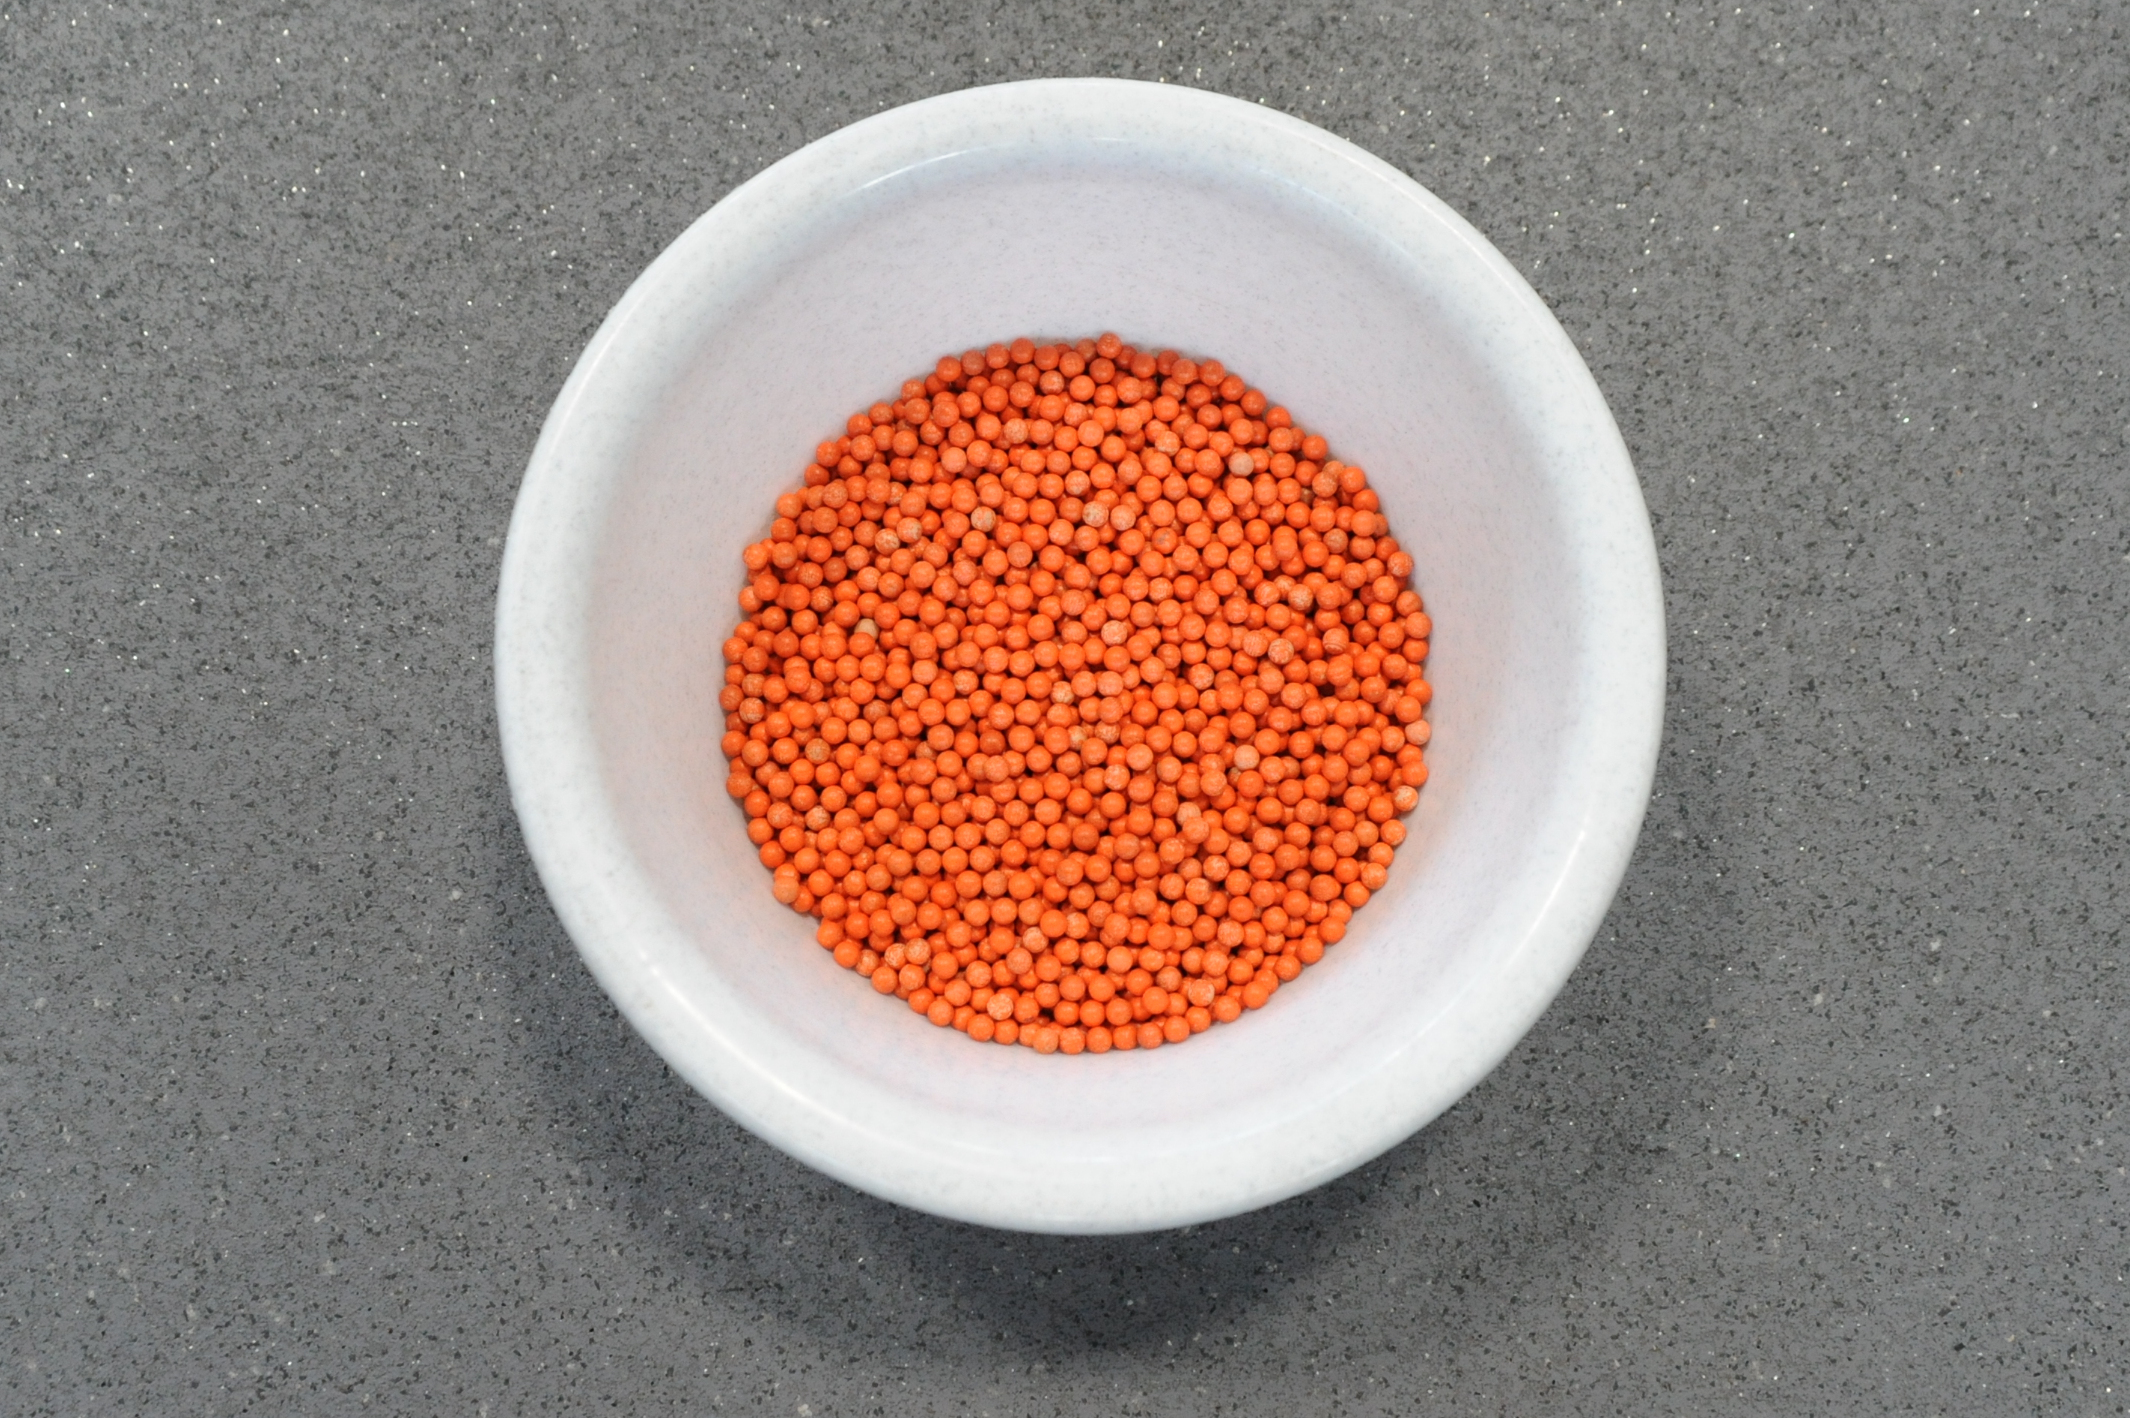
\includegraphics[width=\textwidth]{KugelnCropped2}
		\caption{Spheres}
	\end{subfigure}
	% \hfill
	\quad
	\begin{subfigure}[t]{0.4\textwidth}
		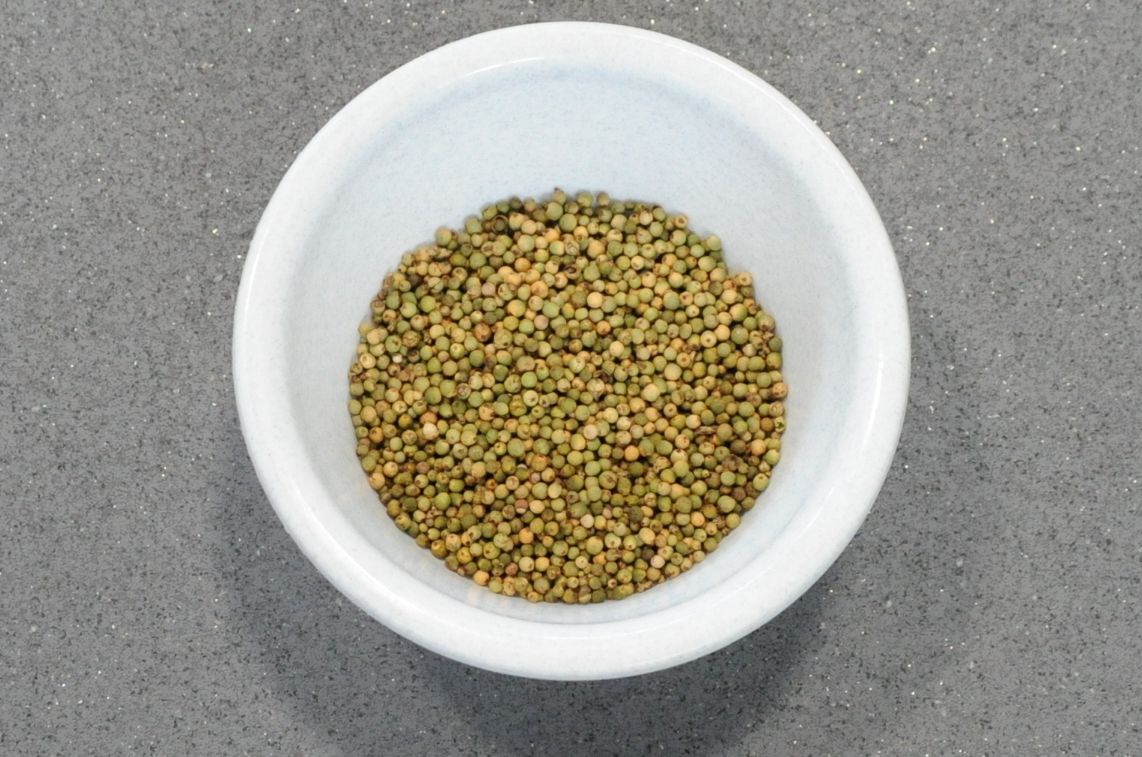
\includegraphics[width=\textwidth]{PfefferCropped2}
		\caption{Peppercorns}
	\end{subfigure}
	\vskip\baselineskip

	\begin{subfigure}[t]{0.4\textwidth}
		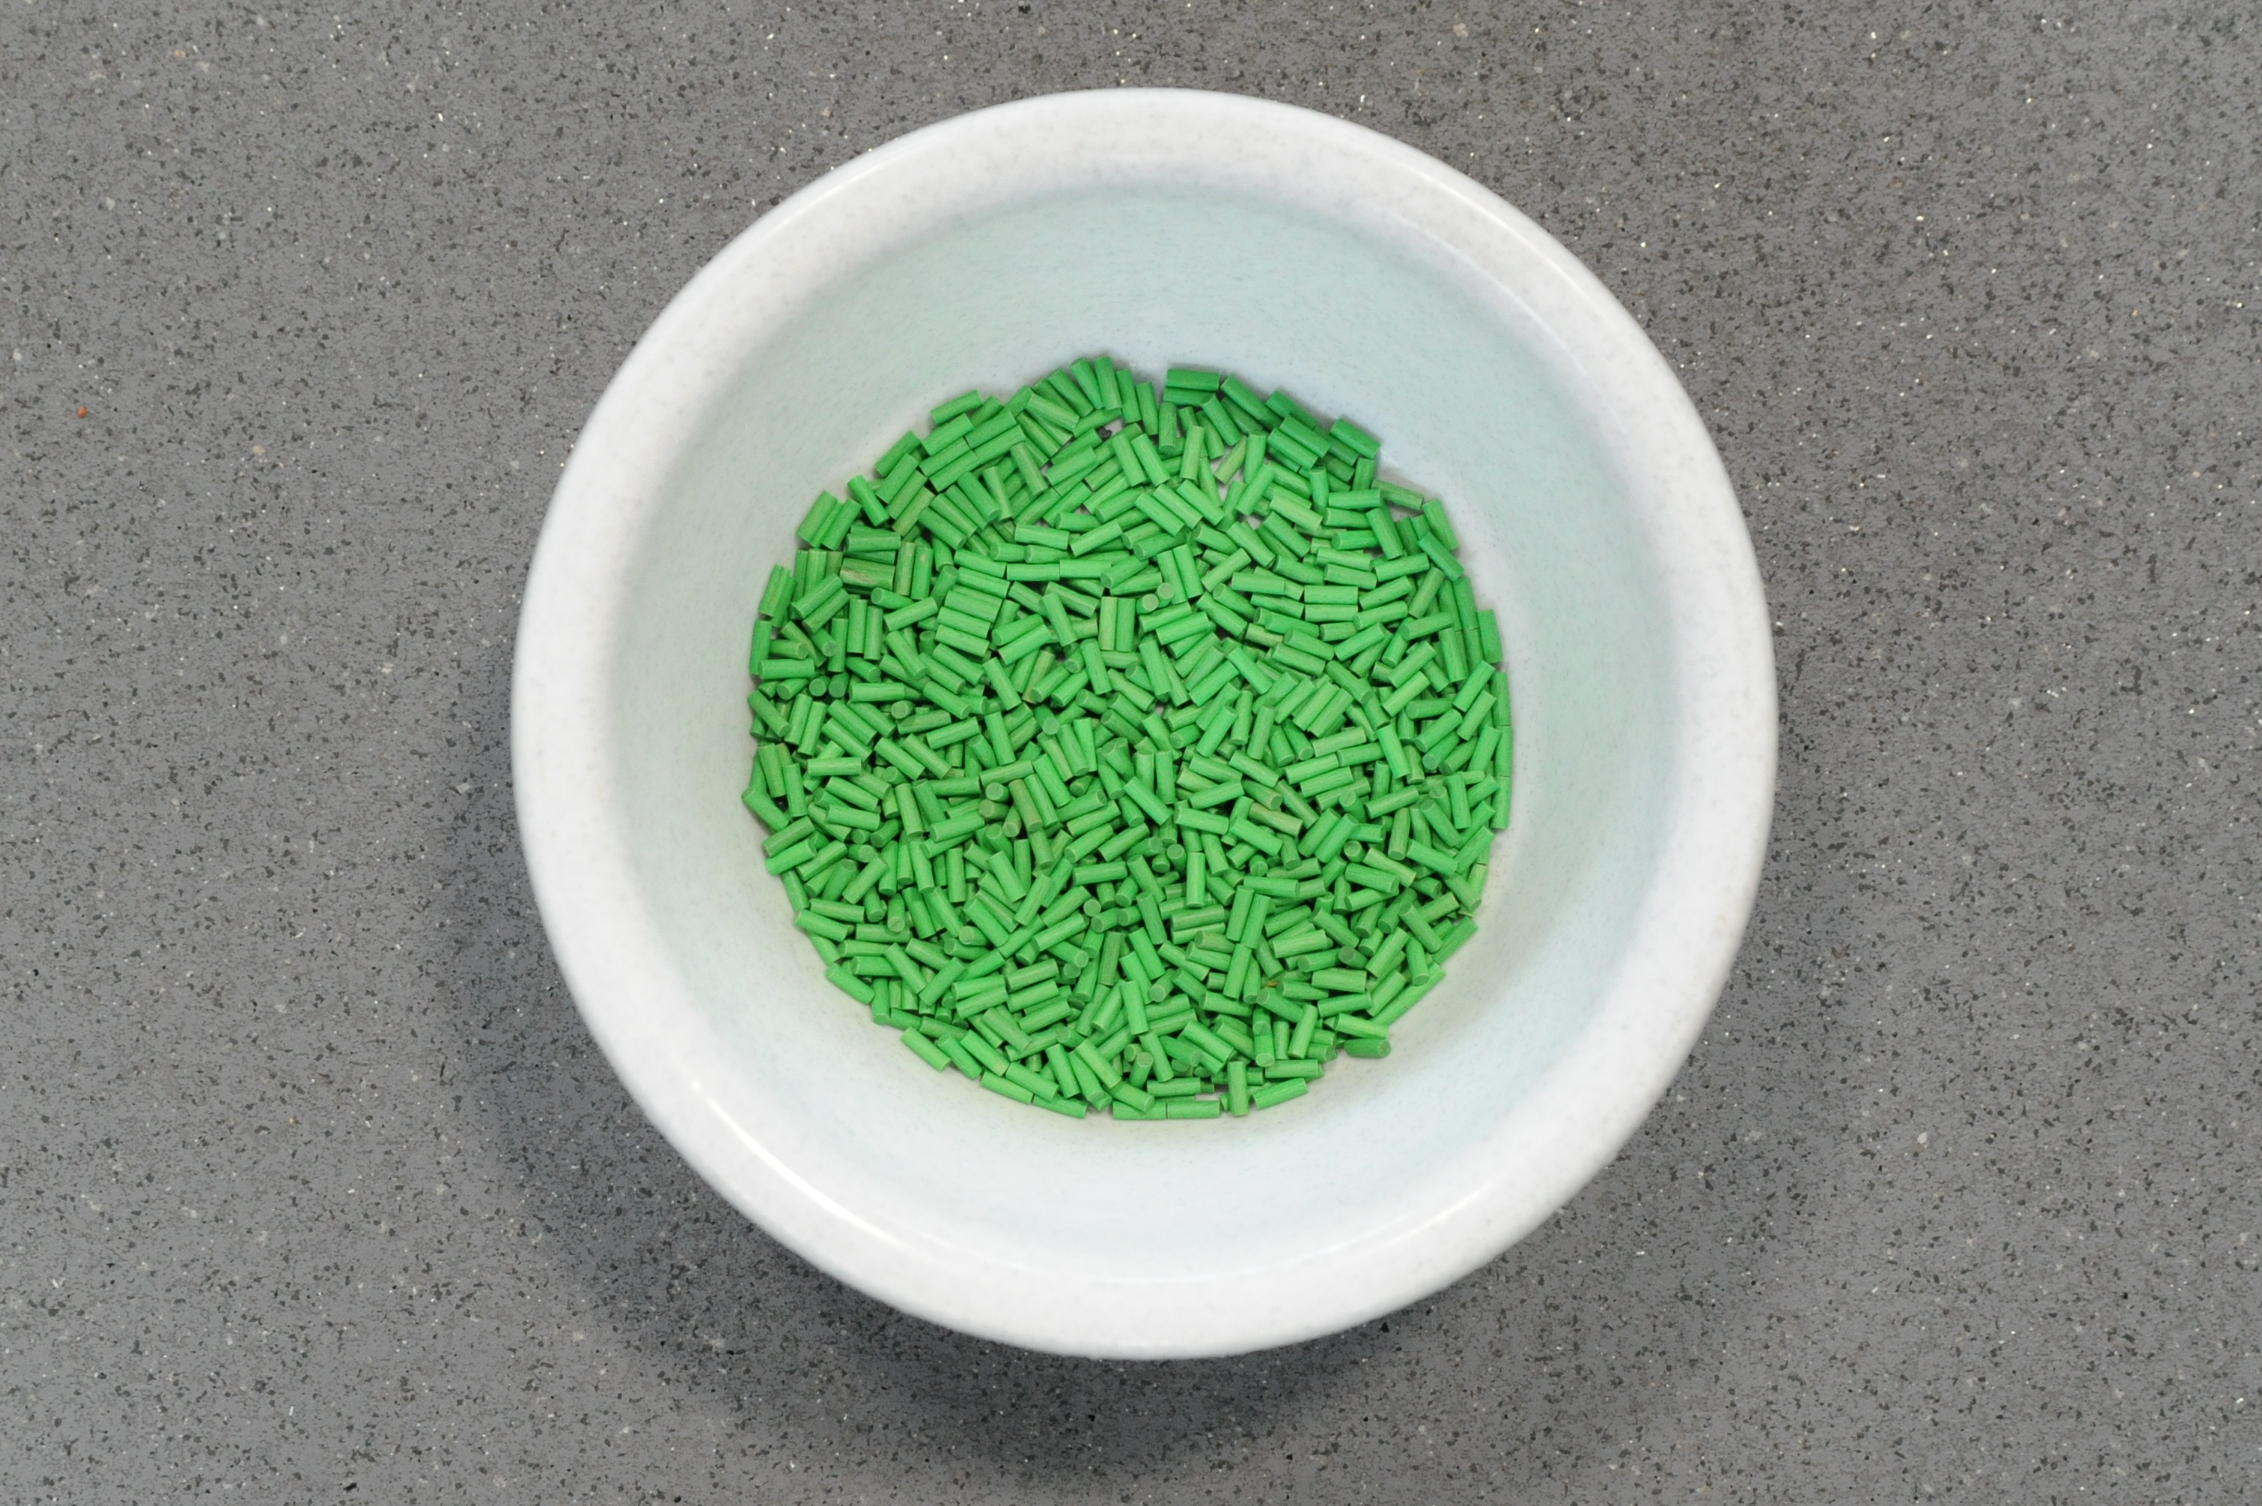
\includegraphics[width=\textwidth]{ZylinderCropped2}
		\caption{Cylinders}
	\end{subfigure}
	\quad
	\begin{subfigure}[t]{0.4\textwidth}
		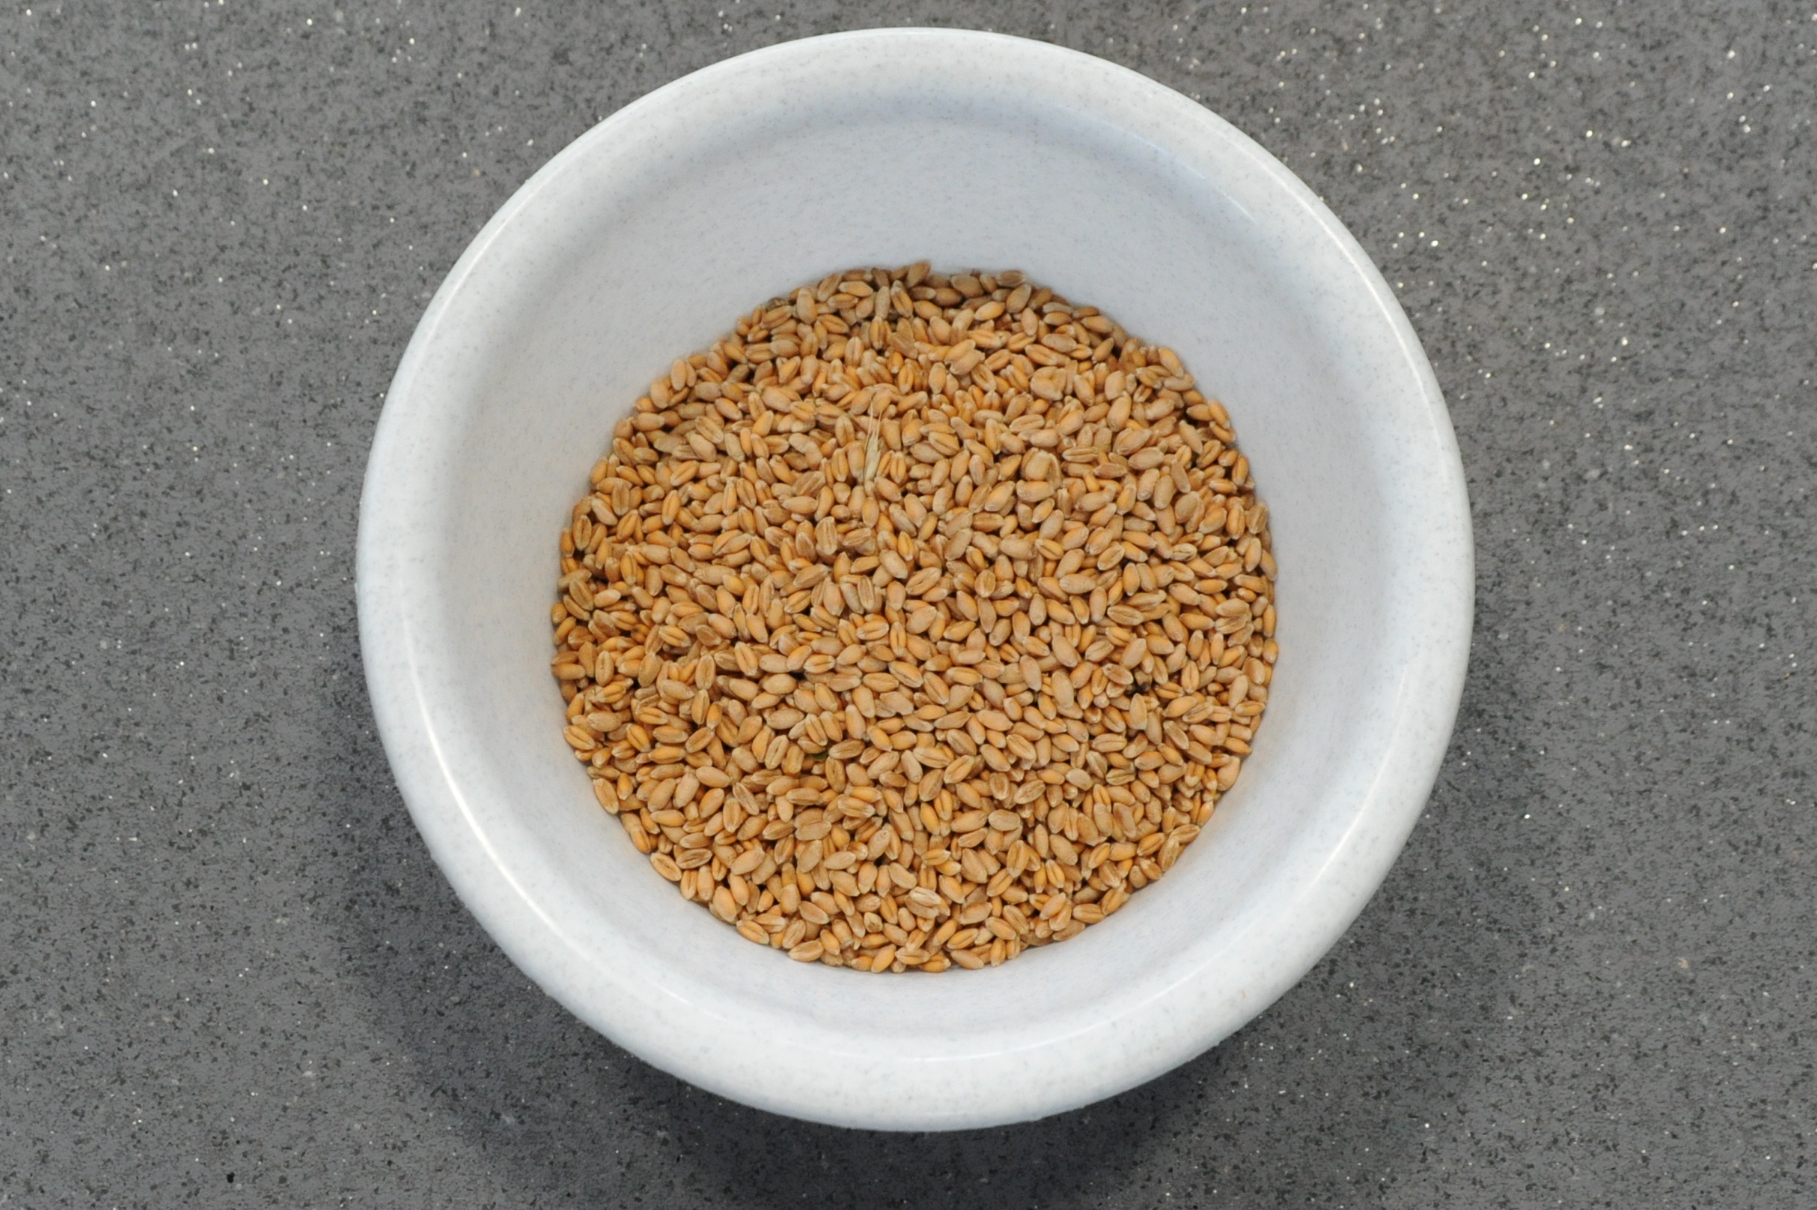
\includegraphics[width=\textwidth]{WeizenCropped2}
		\caption{Wheat grains}
	\end{subfigure}
	\caption{Different materials in the dataset \cite{hornberger2018}.}
	\label{fig:schuettgueterSchuessel}
\end{figure}

As shown in Figure \ref{fig:tablesortsystem}, the camera was assembled above the conveyor belt. The pictures taken by the camera have a resolution of 2320$\times$1726 pixels  \cite{hornberger2018}. Each pixel in the image corresponds approximately to \SI{0.056}{\milli\meter}. The recorded position from the experiment is given in pixels. In the further part of the work, pixels are used as the unit of position for the datasets from real materials.
% average velocity.jpg

The pictures taken in the experiments were later converted into CSV files containing the coordinates of the centers of the particles for each dataset. These CSV files contain the information of measurements in the tracking algorithm. In these CSV files, each line represents an image from a time step. Each line starts with the frame number, followed by the number of particles detected and then the coordinates of the centers of the detected particles. Each coordinate is given in a $1\times 2$ tuple including the coordinate on x-direction $\mathsf{x}$ and y-direction $\mathsf{y}$. In the tracking algorithm, the CSV files are transferred into midpoint matrices, which contain only the coordinate tuples. An example of an excerpt from CSV files can be seen in Table \ref{table:Sample of CSV}. 

% \textcolor{red}{added some information of density, velocity etc.}

The datasets used in this thesis include ten datasets for each material, and each dataset is tested separately in the following experiments. Each dataset contains 3,500 frames. A sphere, peppercorn or wheat grain dataset contains 315\-887 tracks. A cylinder dataset contains 1,101-2,122 tracks. The average velocities of particles in the dataset are between 75-95 pixel/frame. 

The datasets from real materials have no ground truth data. Thus, the last measurement of each track was used for calculating the prediction error. In order to obtain the association information, a reference tracking result was generated with the tracking algorithm from one dataset for each material. The association of each track in the reference tracking result was manually examined to ensure that no association errors appear in the result. Only the dataset with the reference tracking result was used in the grid search for prediction hyperparameters and experiments for association hyperparameters.

\begin{table}[ht]
    \caption{Excerpt from a dataset in .csv format \cite{hornberger2018}.}
	\small
	\centering
    \begin{tabular}{@{}rcrrrrrr@{}}
    \toprule
    Frame   & \#MP & MP\_1\_x  & MP\_1\_y  & MP\_2\_x  & MP\_2\_y  & MP\_3\_x & MP\_3\_y \\ \midrule
    636     & 1    & 1222.9975 & 92.7641   & NaN       & NaN       & NaN      & NaN      \\
    637     & 1    & 1223.4063 & 182.9758  & NaN       & NaN       & NaN      & NaN      \\
    638     & 1    & 1223.6052 & 273.2425  & NaN       & NaN       & NaN      & NaN      \\
    639     & 1    & 1223.7067 & 364.0339  & NaN       & NaN       & NaN      & NaN      \\
    640     & 1    & 1224.0704 & 453.9057  & NaN       & NaN       & NaN      & NaN      \\
    641     & 2    & 1224.2051 & 544.5191  & 1692.4549 & 43.8822   & NaN      & NaN      \\
    642     & 2    & 1224.5793 & 634.7288  & 1696.6901 & 135.9595  & NaN      & NaN      \\
    643     & 2    & 1224.9082 & 726.0094  & 1700.451  & 229.1195  & NaN      & NaN      \\
    644     & 2    & 1225.2296 & 815.9663  & 1704.1472 & 321.2075  & NaN      & NaN      \\
    645     & 2    & 1225.4286 & 906.7078  & 1708.0593 & 414.2785  & NaN      & NaN      \\
    646     & 2    & 1225.7588 & 996.0286  & 1711.5309 & 506.0545  & NaN      & NaN      \\
    647     & 3    & 1226.0411 & 1086.5729 & 1714.8831 & 599.5417  & 961.8821 & 62.7111  \\
    648     & 3    & 1226.2337 & 1175.9271 & 1718.1401 & 691.6325  & 958.5526 & 154.3124 \\
    649     & 3    & 1226.2073 & 1265.7495 & 1721.6618 & 784.5927  & 955.3107 & 246.5241 \\
    650     & 3    & 1226.2543 & 1354.9362 & 1724.9158 & 876.7192  & 952.4919 & 338.1123 \\
    651     & 3    & 1226.2634 & 1444.5903 & 1728.3341 & 970.2909  & 949.2896 & 430.9692 \\
    652     & 3    & 1226.0845 & 1533.0901 & 1732.1745 & 1062.4624 & 946.3455 & 522.8667 \\
    653     & 3    & 1225.7319 & 1621.8461 & 1735.8759 & 1155.2937 & 943.3384 & 615.4545 \\
    654     & 2    & 1739.6714 & 1247.1867 & 940.2511  & 707.7306  & NaN      & NaN      \\
    655     & 2    & 1743.4279 & 1339.4146 & 937.2216  & 800.4557  & NaN      & NaN      \\
    656     & 2    & 1747.1525 & 1430.2501 & 934.5311  & 891.7249  & NaN      & NaN      \\
    657     & 2    & 1750.9771 & 1521.8102 & 931.6626  & 984.2284  & NaN      & NaN      \\
    658     & 2    & 1754.1491 & 1612.5565 & 928.7587  & 1076.4749 & NaN      & NaN      \\
    659     & 1    & 925.8463  & 1168.794  & NaN       & NaN       & NaN      & NaN      \\
    660     & 1    & 922.8752  & 1260.7461 & NaN       & NaN       & NaN      & NaN      \\
    661     & 1    & 920.2056  & 1352.8549 & NaN       & NaN       & NaN      & NaN      \\
    662     & 1    & 917.4051  & 1444.3431 & NaN       & NaN       & NaN      & NaN      \\
    663     & 1    & 914.6493  & 1535.5131 & NaN       & NaN       & NaN      & NaN      \\
    664     & 1    & 911.8565  & 1626.5341 & NaN       & NaN       & NaN      & NaN      \\ \bottomrule
    \end{tabular}
    \normalsize
    
    \label{table:Sample of CSV}
    \end{table}


    
\section{Datasets from Mixture of Real Materials}

% \textcolor{red}{added this section}

The mixed materials used in this thesis are the construction waste containing small particles of bricks and limestones, as shown in Figure \ref{bauschutt}. The experimental settings and data format of the datasets with mixed materials are the same as the homogeneous materials. The average velocities of particles in the dataset are around 65 pixel/frame. 
% This value was also set as the initial velocity guess in the tracking algorithm. 
The mixture material dataset contains three datasets, each with 3500 frames. All three datasets were used in this thesis.

\begin{figure}[htbp]
    \centering
	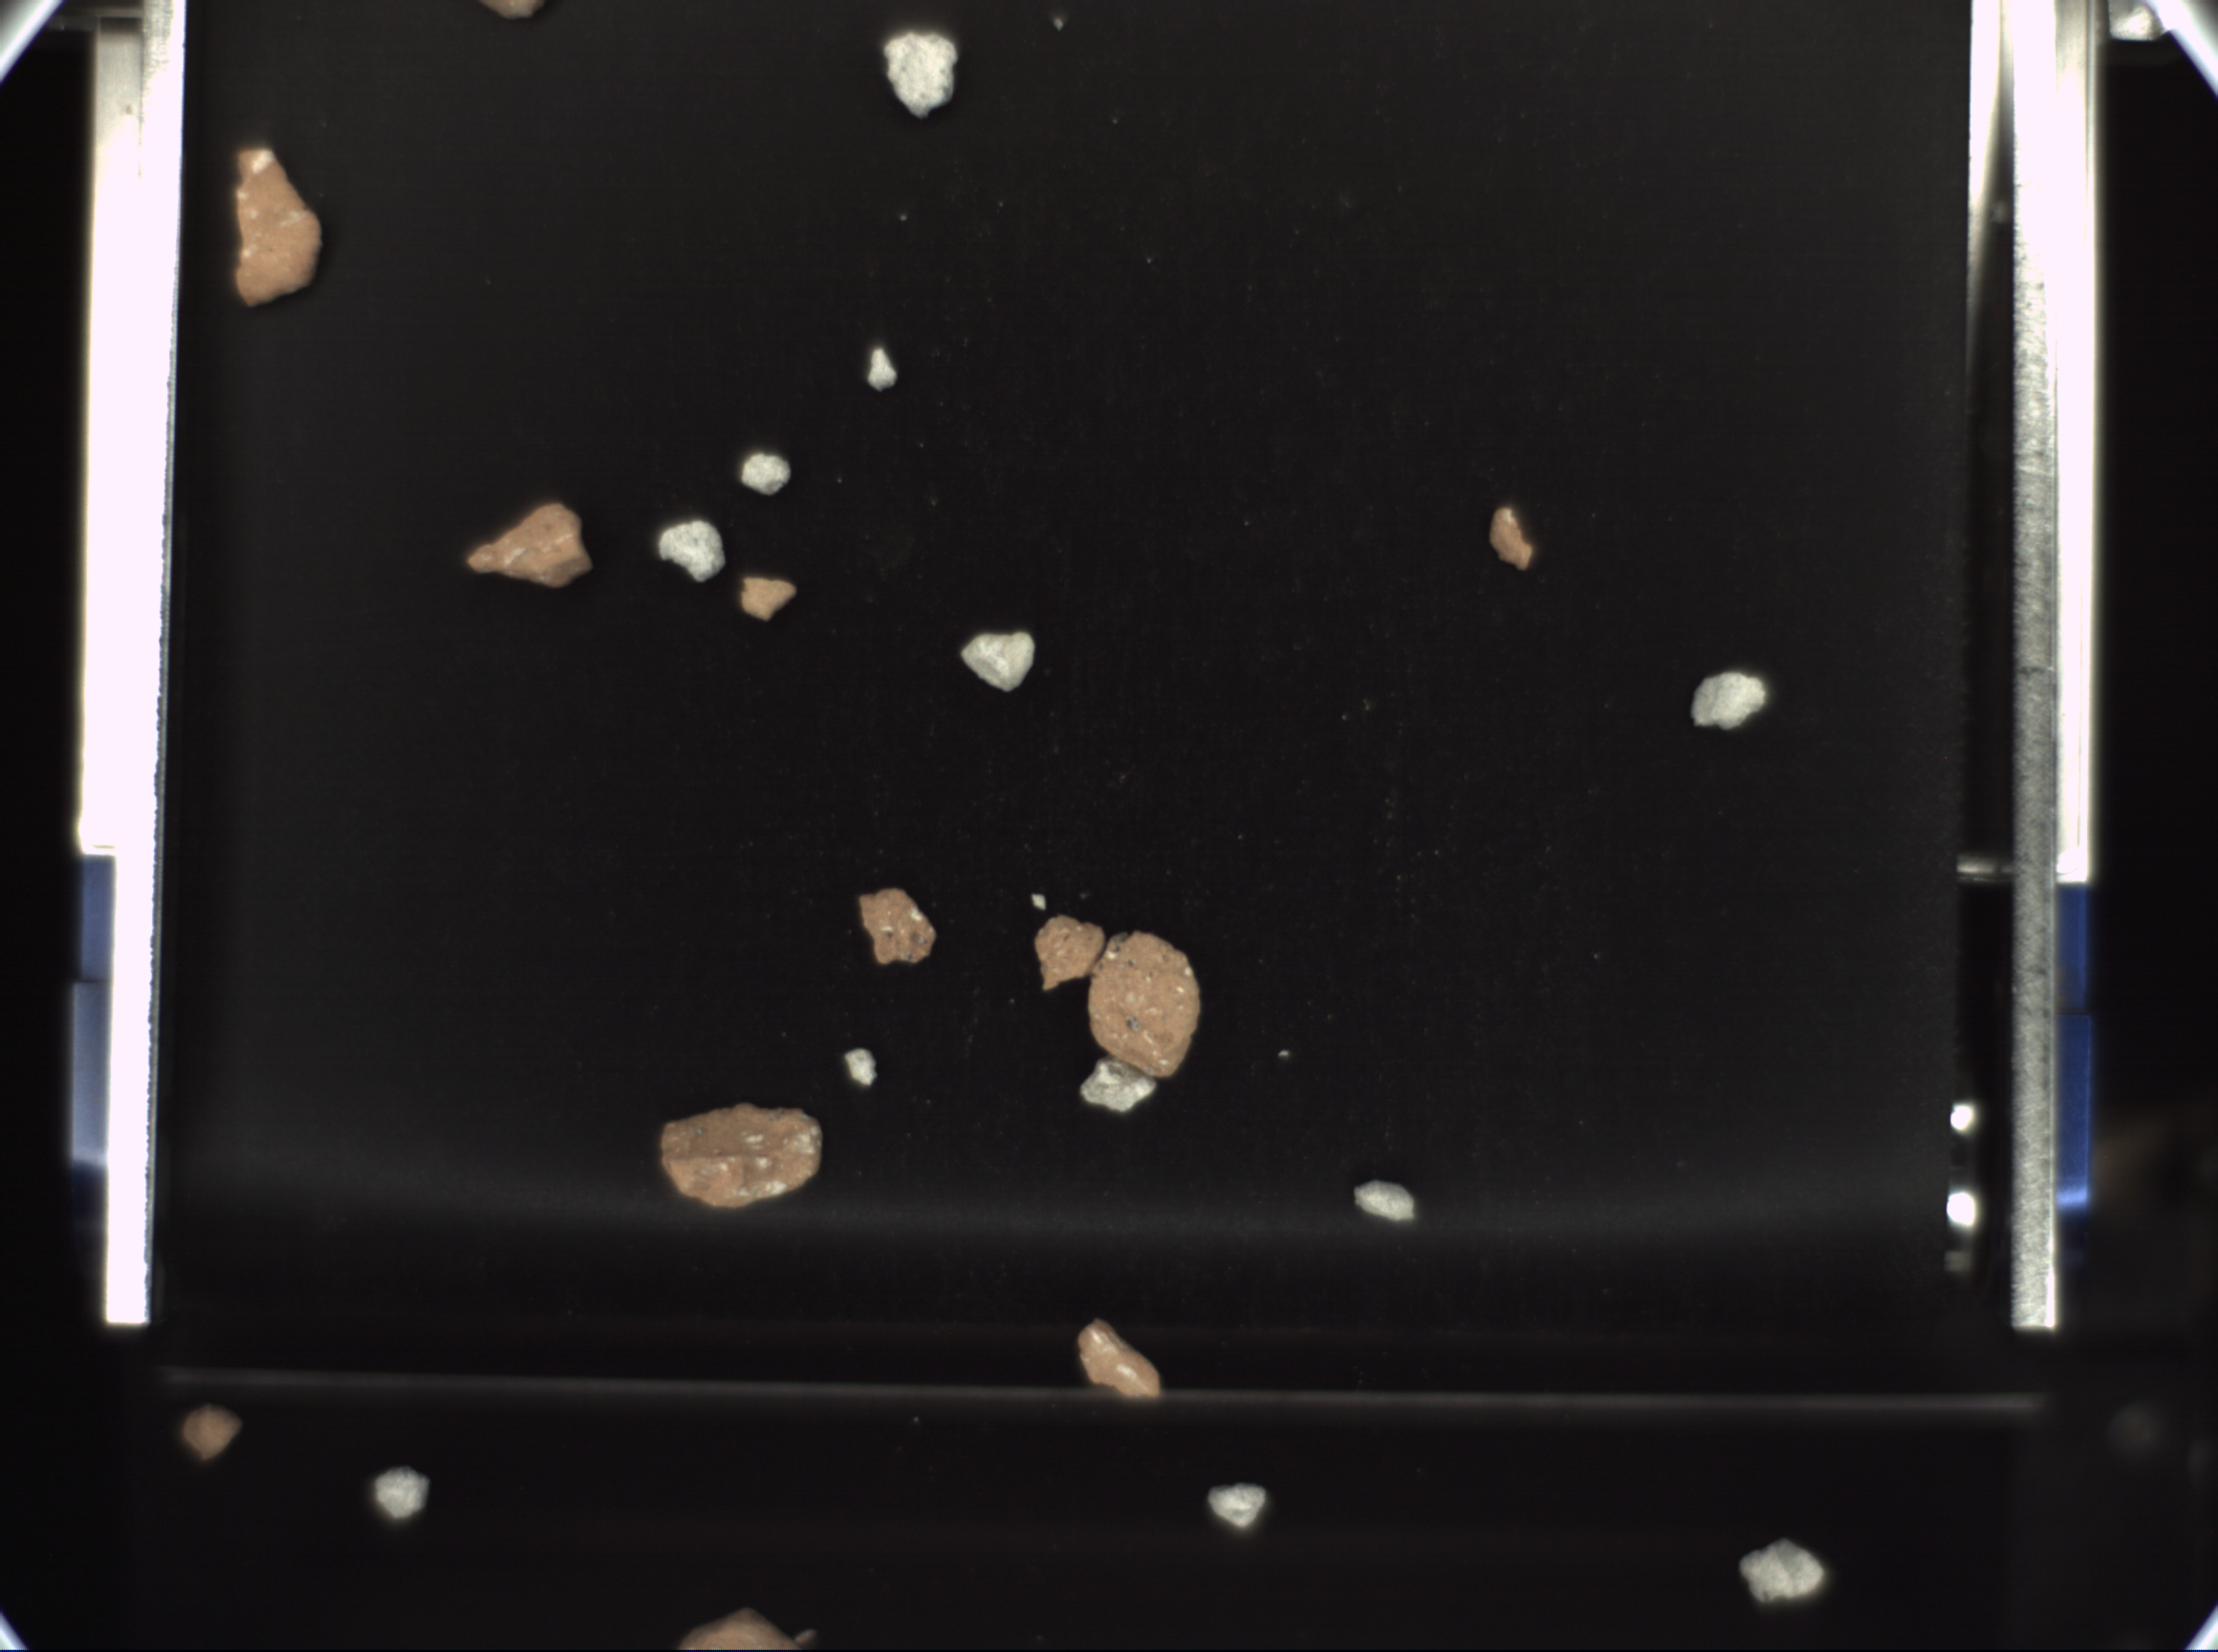
\includegraphics[width=0.6\textwidth]{figures/ZiegelzuKalk50zu50_20gpros00037.png}
	\caption{Mixture of construction wastes, containing particles of bricks and limestones.}
	\label{bauschutt}
\end{figure}


\section{Datasets from Simulation}

In addition to the datasets based on real experiments, some simulated data were also used in this work. \cite{pieper2016numerical} and \cite{pieper2017numerical} show how these datasets were created based on a highly accurate numerical simulation of the \textit{TableSort} system using the discrete element method. The forces acting on the individual particles were calculated numerically based on their condition and the relevant physical laws. Because all the data came from the simulation, the data represent the exact motion of the simulated particles. Thus, all the measurements in the dataset can be seen as the ground truth data and contain no measurement error.

Figure \ref{fig:DEMSimulation} shows the virtual structure of the bulk material sorter on which the simulation was carried out. The position data in the datasets were originally sampled with a frequency of \SI{1000}{\hertz}. However, in order to reduce the size of the dataset and accelerate the tracking process, the frequency was reduced to \SI{100}{\hertz} in the datasets for the experiments in this thesis. The dataset from the simulation is given directly in midpoint matrices in \textsc{Matlab}.

The position information of the simulation is given in meters. The transport direction of the conveyor belt is along the \(\mathsf {x}\) axis. The conveyor belt extends along the \(\mathsf{y} \) axis from \SI{0.0}{\meter} to \SI{0.18}{\meter} and along the \(\mathsf{x}\) - Axis from \SI{0.388}{\meter} to \SI{0.788}{\meter}. The average velocities of particles in the dataset are around \SI{1}{\metre\per\second}, or \SI{0.01}{\metre\per}/frame. The DEM dataset contains 3,713 tracks in 2,000 frames. 

\begin{figure}[htb]
    \centering
	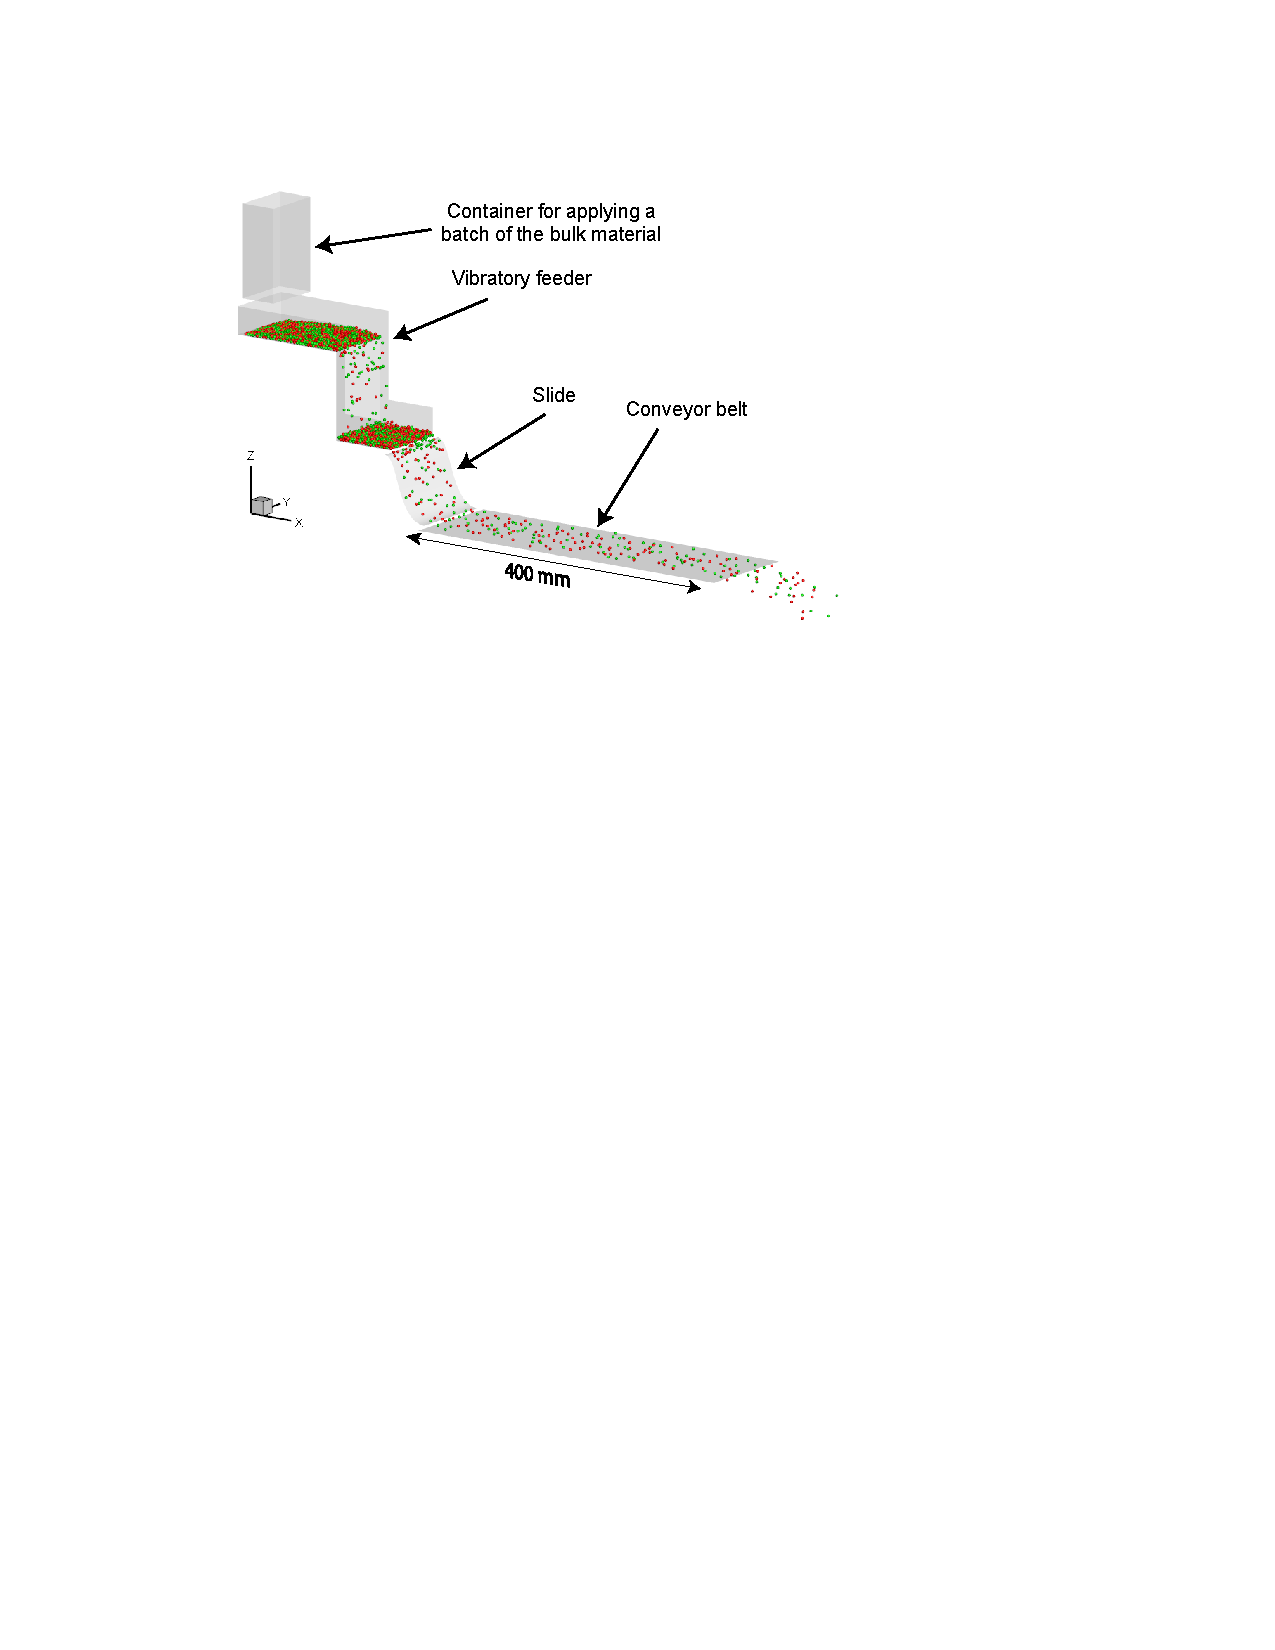
\includegraphics[width=0.8\textwidth]{DEM-Sim}
	\caption{Visualization of the DEM simulation \cite{pfaff2019multitarget}.}
	\label{fig:DEMSimulation}
\end{figure}





\section{Artificial Datasets}
\label{Artificial Datasets}

% \textcolor{red}{added details}

Besides the dataset mentioned above, some simple datasets were generated for the validation of the optimization methods. These datasets were generated according to the motion models mentioned in \Sec{Motion Models}. All the hyperparameters, including the initial velocity and the variances for each state variables, were given before the generation of the artificial dataset. In the validation, the optimization algorithm should reconstruct these hyperparameters. The hyperparameter values for the generation of the datasets are listed in Table \ref{defaultCVvali} and \ref{defaultCVAvali}. In order to avoid the interference of the association errors in the validation, the dataset contains only one track at the same time. The dataset contains 10000 tracks in total, where each track contains 20 measurements.

\begin{table}[htbp] 
    \centering
    \caption{List of the value of the hyperparameters in CV model for artificial datasets.} 
    \begin{tabular}{ccc} 
    \toprule 
    Hyperparameters&Notation& Default value\\ 
    \midrule 
    Initial velocity guess              &$v_{0}$&100\\
    Initial position variance           &$S_{\mathrm{pos}}^{\mathrm{ini}}$&0.5\\
    Initial velocity variance           &$S_{\mathrm{vel}}^{\mathrm{ini}}$&0.2\\
    Refined initial velocity variance   &$S_{\mathrm{vel}}^{\mathrm{ini, r}}$&0.2\\
    Measurement variance                &$S^{\boldsymbol{v}}$&0.2\\
    System noise variance               &$S^{\boldsymbol{w}}$&0.1\\ 
    \bottomrule 
    \end{tabular} 
    \label{defaultCVvali}
\end{table}

\begin{table}[htb] 
    \centering
    \caption{List of the value of the hyperparameters in CVA model for generating the artificial datasets.} 
    \begin{tabular}{ccc} 
    \toprule 
    Hyperparameters&Notation& Value\\ 
    \midrule 
    Initial velocity guess              &$v_{0}$&100\\
    Initial position variance           &$S_{\mathrm{pos}}^{\mathrm{ini}}$&0.5\\
    Initial velocity variance           &$S_{\mathrm{vel}}^{\mathrm{ini}}$&0.2\\
    Refined initial velocity variance   &$S_{\mathrm{vel}}^{\mathrm{ini, r}}$&0.2\\
    Initial angle variance              &$S_{\mathrm{ang}}^{\mathrm{ini}}$&0.1\\
    Measurement position variance       &$S_{\mathrm{pos}}^{\boldsymbol{v}}$&0.2\\
    Measurement velocity variance       &$S_{\mathrm{vel}}^{\boldsymbol{v}}$&0.2\\
    Measurement angle variance          &$S_{\mathrm{ang}}^{\boldsymbol{v}}$&0.1\\
    Prediction position variance        &$S_{\mathrm{pos}}^{\boldsymbol{w}}$&0.1\\
    Prediction velocity variance        &$S_{\mathrm{vel}}^{\boldsymbol{w}}$&0.2\\
    Prediction angle variance           &$S_{\mathrm{ang}}^{\boldsymbol{w}}$&0.1\\
    \bottomrule 
    \end{tabular} 
    \label{defaultCVAvali}
\end{table}

% These datasets served only for the validation of the optimization of the hyperparameters for motion prediction.  The optimization for each hyperparameter is performed with ten datasets in the same setting, and the final optimized value is taken as the average of all the ten optimization results.